\subsection{Generic APIs vs Consumer Driven APIs}\label{subsection:background:micro-frontend:generic-vs-consumer-driven-apis}

The big decision in micro-frontend \ac{API} development is to use either generic or consumer-oriented \acp{API}. The difference is that generic \acp{API} emphasize reusability, while consumer-oriented \acp{API} tailor the \acp{API} to the customer.

\subsubsection{Generic \acp{API}}\label{subsubsection:background:micro-frontend:generic-vs-consumer-driven-apis:generic-apis}

Generic \acp{API} refer to \acp{API} that are very general and can be used by different clients. However, this type of \ac{API} has two significant drawbacks. Over-fetching describes the problem of getting more data than is needed, and Over-requesting describes the problem of needing multiple requests to get the data for a use case. Both problems are discussed in more detail in the following paragraphs. \cite{misc:2019:leitner:background:micro-frontends:backend-for-frontends}

\paragraph{Over-Fetching}\label{paragraph:background:micro-frontend:generic-vs-consumer-driven-apis:generic-apis:over-fetching}

For example, a contact service provides a contact model that includes \texttt{customerNumber}, \texttt{firstName}, \texttt{secondName}, \texttt{uidNumber}, and the user's address, as seen in the Listing \ref{code:background:micro-frontends:over-fetching}. However, one application requirement is to display only a contact's first and last name inside the header. Only two fields of the model are used, and the rest are unnecessarily queried. \cite{misc:2019:leitner:background:micro-frontends:backend-for-frontends}

\ifshowListings
\begin{listing}[H]
  \begin{minted}{typescript}
interface ContactModel {
  id: string;
  customerNumber: string;
  firstName: string;
  secondName: string;
  uidNumber: string;

  Address: {
    id: string;
    postalCode: string;
    location: string;
    Country: string;
  }
}
  \end{minted}
  \caption{Contact-Model that contains too many fields for a use-case.}\label{code:background:micro-frontends:over-fetching}
\end{listing}
\fi

\paragraph{Over-Requesting}\label{paragraph:background:micro-frontend:generic-vs-consumer-driven-apis:generic-apis:over-requesting}

Attempting to solve the problem of over-fetching by reducing the amount of data set that is returned leads directly to this problem. Listing \ref{code:background:micro-frontends:over-requesting} shows the problem of over-requesting. If another requirement inside the application should display the address alongside the contact, two requests have to be performed every time. Afterwards, the two data sets have to be merged, leading to high client complexity. \cite{misc:2019:leitner:background:micro-frontends:backend-for-frontends}

\ifshowListings
\begin{listing}[H]
  \begin{minted}{typescript}
interface ContactModel {
  id: string;
  customerNumber: string;
  firstName: string;
  secondName: string;
  uidNumber: string;

  address_id: string;
}
  \end{minted}
  \caption{Contact-Model model that links to the address-model with the address id.}\label{code:background:micro-frontends:over-requesting}
\end{listing}
\fi

\subsubsection{Consumer Driven \acp{API}}\label{subsubection:background:micro-frontend:generic-vs-consumer-driven-apis:consumer-driven-apis}

Consumer-driven \acp{API} are the opposite of generic \acp{API}. They follow the idea of providing the client with exactly the data it needs. Following the example above, the contact service would have an endpoint that returns only the first and last name as required for the request. These endpoints make communication with a client straightforward, and there is no problem of over-fetching and over-requesting. However, creating an endpoint for each request creates an unmanageable set of endpoints.  \cite{misc:2019:leitner:background:micro-frontends:backend-for-frontends} To solve the problems of over-fetching and over-requesting, the \ac{BFF} pattern is often used. This pattern provides each client with their own \ac{API}, which is adapted to their needs. \cite{book:2018:richardson:background:bff:microservices-patterns}

\ifshowImages
\begin{figure}[H]
  \centering
  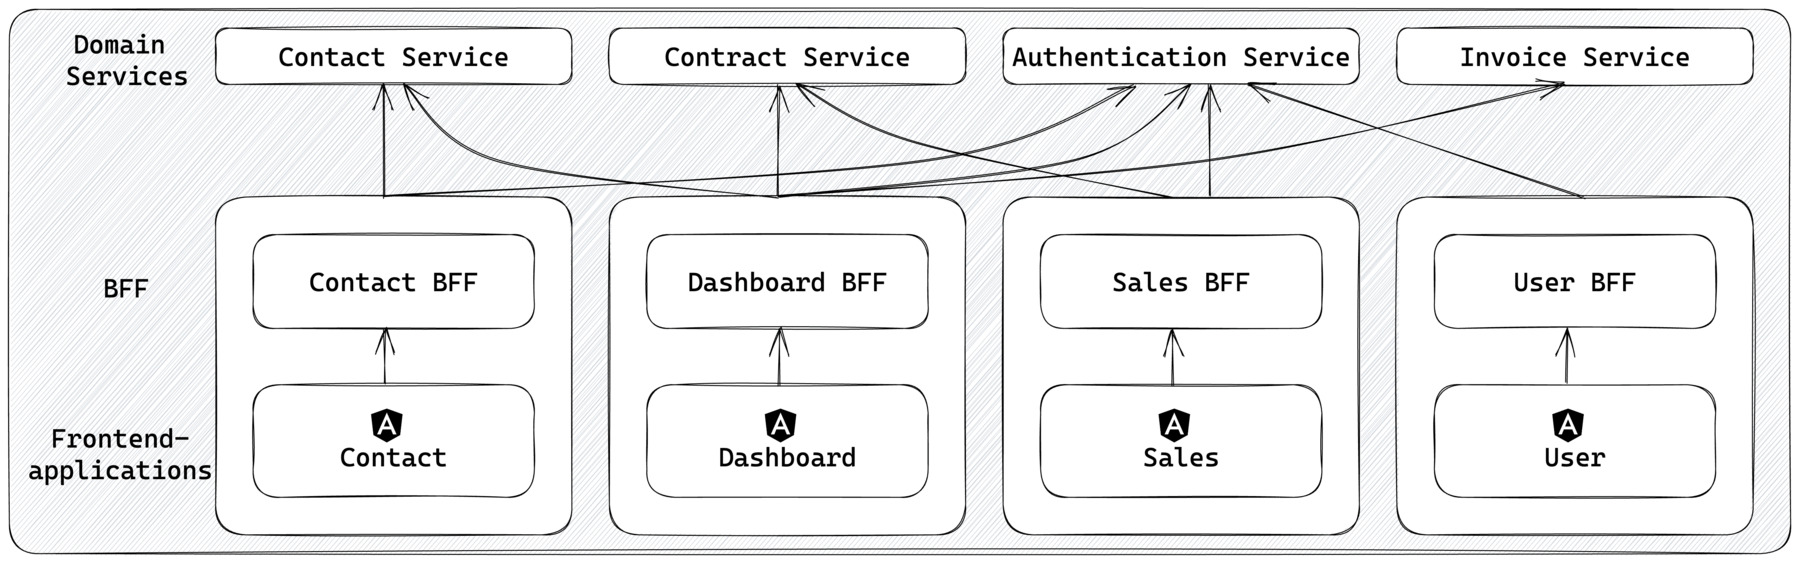
\includegraphics[width=1\linewidth]{images/background/micro-frontends/bff-architecture.jpg}
  \caption{A frontend architecture using the \ac{BFF} pattern.}\label{fig:background:micro-frontend:bff-architecture}
\end{figure}
\fi

\noindent Figure \ref{fig:background:micro-frontend:bff-architecture} shows an exemplary micro-frontend architecture using the \ac{BFF} pattern. Each frontend has a service that retrieves data only for that specific client. Because the \acp{BFF} function as a gateway to the domain services, the domain services can stay very generic and be reused by different clients. \acp{BFF} should implement only the presentation logic that puts the data into the form that the client needs, and it should avoid storing state. \cite{misc:2019:leitner:background:micro-frontends:backend-for-frontends}

\bigskip

\noindent With this architectural approach, the \ac{BFF} and the frontend form a single deployment unit. If one application changes, the other must adapt to the changes. GraphQL is a perfect technology for implementing a \ac{BFF} because it is specifically designed for implementing the presentation layer.
